% Options for packages loaded elsewhere
\PassOptionsToPackage{unicode}{hyperref}
\PassOptionsToPackage{hyphens}{url}
%
\documentclass[
]{article}
\usepackage{lmodern}
\usepackage{amssymb,amsmath}
\usepackage{ifxetex,ifluatex}
\ifnum 0\ifxetex 1\fi\ifluatex 1\fi=0 % if pdftex
  \usepackage[T1]{fontenc}
  \usepackage[utf8]{inputenc}
  \usepackage{textcomp} % provide euro and other symbols
\else % if luatex or xetex
  \usepackage{unicode-math}
  \defaultfontfeatures{Scale=MatchLowercase}
  \defaultfontfeatures[\rmfamily]{Ligatures=TeX,Scale=1}
\fi
% Use upquote if available, for straight quotes in verbatim environments
\IfFileExists{upquote.sty}{\usepackage{upquote}}{}
\IfFileExists{microtype.sty}{% use microtype if available
  \usepackage[]{microtype}
  \UseMicrotypeSet[protrusion]{basicmath} % disable protrusion for tt fonts
}{}
\makeatletter
\@ifundefined{KOMAClassName}{% if non-KOMA class
  \IfFileExists{parskip.sty}{%
    \usepackage{parskip}
  }{% else
    \setlength{\parindent}{0pt}
    \setlength{\parskip}{6pt plus 2pt minus 1pt}}
}{% if KOMA class
  \KOMAoptions{parskip=half}}
\makeatother
\usepackage{xcolor}
\IfFileExists{xurl.sty}{\usepackage{xurl}}{} % add URL line breaks if available
\IfFileExists{bookmark.sty}{\usepackage{bookmark}}{\usepackage{hyperref}}
\hypersetup{
  pdftitle={Statistical Inference - Inferential Data Analysis},
  pdfauthor={Ivan Jennings},
  hidelinks,
  pdfcreator={LaTeX via pandoc}}
\urlstyle{same} % disable monospaced font for URLs
\usepackage[margin=1in]{geometry}
\usepackage{color}
\usepackage{fancyvrb}
\newcommand{\VerbBar}{|}
\newcommand{\VERB}{\Verb[commandchars=\\\{\}]}
\DefineVerbatimEnvironment{Highlighting}{Verbatim}{commandchars=\\\{\}}
% Add ',fontsize=\small' for more characters per line
\usepackage{framed}
\definecolor{shadecolor}{RGB}{248,248,248}
\newenvironment{Shaded}{\begin{snugshade}}{\end{snugshade}}
\newcommand{\AlertTok}[1]{\textcolor[rgb]{0.94,0.16,0.16}{#1}}
\newcommand{\AnnotationTok}[1]{\textcolor[rgb]{0.56,0.35,0.01}{\textbf{\textit{#1}}}}
\newcommand{\AttributeTok}[1]{\textcolor[rgb]{0.77,0.63,0.00}{#1}}
\newcommand{\BaseNTok}[1]{\textcolor[rgb]{0.00,0.00,0.81}{#1}}
\newcommand{\BuiltInTok}[1]{#1}
\newcommand{\CharTok}[1]{\textcolor[rgb]{0.31,0.60,0.02}{#1}}
\newcommand{\CommentTok}[1]{\textcolor[rgb]{0.56,0.35,0.01}{\textit{#1}}}
\newcommand{\CommentVarTok}[1]{\textcolor[rgb]{0.56,0.35,0.01}{\textbf{\textit{#1}}}}
\newcommand{\ConstantTok}[1]{\textcolor[rgb]{0.00,0.00,0.00}{#1}}
\newcommand{\ControlFlowTok}[1]{\textcolor[rgb]{0.13,0.29,0.53}{\textbf{#1}}}
\newcommand{\DataTypeTok}[1]{\textcolor[rgb]{0.13,0.29,0.53}{#1}}
\newcommand{\DecValTok}[1]{\textcolor[rgb]{0.00,0.00,0.81}{#1}}
\newcommand{\DocumentationTok}[1]{\textcolor[rgb]{0.56,0.35,0.01}{\textbf{\textit{#1}}}}
\newcommand{\ErrorTok}[1]{\textcolor[rgb]{0.64,0.00,0.00}{\textbf{#1}}}
\newcommand{\ExtensionTok}[1]{#1}
\newcommand{\FloatTok}[1]{\textcolor[rgb]{0.00,0.00,0.81}{#1}}
\newcommand{\FunctionTok}[1]{\textcolor[rgb]{0.00,0.00,0.00}{#1}}
\newcommand{\ImportTok}[1]{#1}
\newcommand{\InformationTok}[1]{\textcolor[rgb]{0.56,0.35,0.01}{\textbf{\textit{#1}}}}
\newcommand{\KeywordTok}[1]{\textcolor[rgb]{0.13,0.29,0.53}{\textbf{#1}}}
\newcommand{\NormalTok}[1]{#1}
\newcommand{\OperatorTok}[1]{\textcolor[rgb]{0.81,0.36,0.00}{\textbf{#1}}}
\newcommand{\OtherTok}[1]{\textcolor[rgb]{0.56,0.35,0.01}{#1}}
\newcommand{\PreprocessorTok}[1]{\textcolor[rgb]{0.56,0.35,0.01}{\textit{#1}}}
\newcommand{\RegionMarkerTok}[1]{#1}
\newcommand{\SpecialCharTok}[1]{\textcolor[rgb]{0.00,0.00,0.00}{#1}}
\newcommand{\SpecialStringTok}[1]{\textcolor[rgb]{0.31,0.60,0.02}{#1}}
\newcommand{\StringTok}[1]{\textcolor[rgb]{0.31,0.60,0.02}{#1}}
\newcommand{\VariableTok}[1]{\textcolor[rgb]{0.00,0.00,0.00}{#1}}
\newcommand{\VerbatimStringTok}[1]{\textcolor[rgb]{0.31,0.60,0.02}{#1}}
\newcommand{\WarningTok}[1]{\textcolor[rgb]{0.56,0.35,0.01}{\textbf{\textit{#1}}}}
\usepackage{graphicx,grffile}
\makeatletter
\def\maxwidth{\ifdim\Gin@nat@width>\linewidth\linewidth\else\Gin@nat@width\fi}
\def\maxheight{\ifdim\Gin@nat@height>\textheight\textheight\else\Gin@nat@height\fi}
\makeatother
% Scale images if necessary, so that they will not overflow the page
% margins by default, and it is still possible to overwrite the defaults
% using explicit options in \includegraphics[width, height, ...]{}
\setkeys{Gin}{width=\maxwidth,height=\maxheight,keepaspectratio}
% Set default figure placement to htbp
\makeatletter
\def\fps@figure{htbp}
\makeatother
\setlength{\emergencystretch}{3em} % prevent overfull lines
\providecommand{\tightlist}{%
  \setlength{\itemsep}{0pt}\setlength{\parskip}{0pt}}
\setcounter{secnumdepth}{-\maxdimen} % remove section numbering

\title{Statistical Inference - Inferential Data Analysis}
\author{Ivan Jennings}
\date{}

\begin{document}
\maketitle

\hypertarget{overview}{%
\subsection{Overview}\label{overview}}

Analysis of the ToothGrowth data set within the R package. We're going
to perform some basic exploratory data analysis as well as using
confidence intervals and/or hypothesis tests to compare tooth growth by
supp and dose.

\begin{Shaded}
\begin{Highlighting}[]
\KeywordTok{options}\NormalTok{(}\DataTypeTok{scipen=}\DecValTok{999}\NormalTok{)}
\KeywordTok{library}\NormalTok{(dplyr)}
\KeywordTok{library}\NormalTok{(lattice)}
\end{Highlighting}
\end{Shaded}

\hypertarget{loading-and-reviewing-data}{%
\subsection{Loading and reviewing
data}\label{loading-and-reviewing-data}}

First, let's run a few commands to load the data and see how it is
structured.

\begin{Shaded}
\begin{Highlighting}[]
\KeywordTok{data}\NormalTok{(}\StringTok{"ToothGrowth"}\NormalTok{)}
\KeywordTok{str}\NormalTok{(ToothGrowth)}
\end{Highlighting}
\end{Shaded}

\begin{verbatim}
## 'data.frame':    60 obs. of  3 variables:
##  $ len : num  4.2 11.5 7.3 5.8 6.4 10 11.2 11.2 5.2 7 ...
##  $ supp: Factor w/ 2 levels "OJ","VC": 2 2 2 2 2 2 2 2 2 2 ...
##  $ dose: num  0.5 0.5 0.5 0.5 0.5 0.5 0.5 0.5 0.5 0.5 ...
\end{verbatim}

We can see that there are 60 observations of three variables, len, supp
and dose. Let's also take a look at the summary of the data.

\begin{Shaded}
\begin{Highlighting}[]
\KeywordTok{summary}\NormalTok{(ToothGrowth)}
\end{Highlighting}
\end{Shaded}

\begin{verbatim}
##       len        supp         dose      
##  Min.   : 4.20   OJ:30   Min.   :0.500  
##  1st Qu.:13.07   VC:30   1st Qu.:0.500  
##  Median :19.25           Median :1.000  
##  Mean   :18.81           Mean   :1.167  
##  3rd Qu.:25.27           3rd Qu.:2.000  
##  Max.   :33.90           Max.   :2.000
\end{verbatim}

The summary above along with the documentation of the data set in r
using the function ?ToothGrowth gives us an overview of the data that we
are looking at. Here's the description from the R documentation:

\emph{``The response is the length of odontoblasts (cells responsible
for tooth growth) in 60 guinea pigs. Each animal received one of three
dose levels of vitamin C (0.5, 1, and 2 mg/day) by one of two delivery
methods, orange juice or ascorbic acid (a form of vitamin C and coded as
VC).''}

\hypertarget{exploratory-analysis}{%
\subsection{Exploratory Analysis}\label{exploratory-analysis}}

Here is a plot of the data in a graph for us to get an idea of how the
data looks:

\begin{Shaded}
\begin{Highlighting}[]
\KeywordTok{xyplot}\NormalTok{(len }\OperatorTok{~}\StringTok{ }\NormalTok{supp }\OperatorTok{|}\StringTok{ }\KeywordTok{factor}\NormalTok{(dose),}
       \DataTypeTok{data =}\NormalTok{ ToothGrowth,}
       \DataTypeTok{layout =} \KeywordTok{c}\NormalTok{(}\DecValTok{3}\NormalTok{,}\DecValTok{1}\NormalTok{),}
       \DataTypeTok{xlab =} \StringTok{"Delivery Method"}\NormalTok{,}
       \DataTypeTok{ylab =} \StringTok{"Length of Odontoblasts"}\NormalTok{,}
       \DataTypeTok{labels =} \KeywordTok{c}\NormalTok{(}\DecValTok{1}\NormalTok{,}\DecValTok{2}\NormalTok{,}\DecValTok{3}\NormalTok{)}
\NormalTok{       )}
\end{Highlighting}
\end{Shaded}

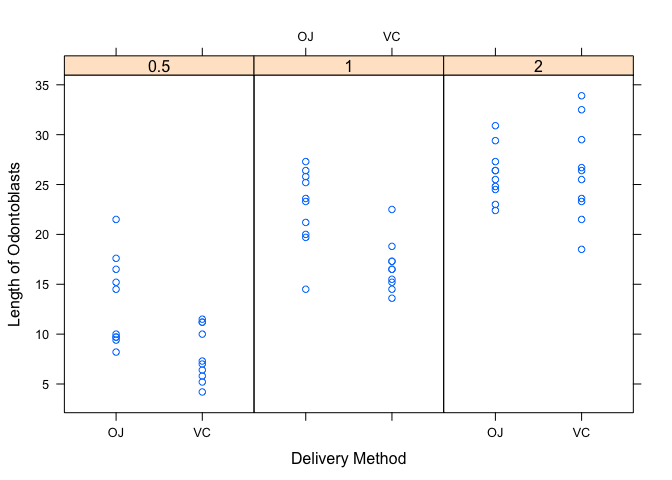
\includegraphics{Statistical_Inference_Part2_files/figure-latex/unnamed-chunk-3-1.pdf}

The above plot shows us each dosage (0.5, 1, 2) and each delivery method
(OJ = Orange Juice, VC = Ascorbic Acid)

We can see from the plot that as the dosage increases, the tooth length
increases as well. We can also see that for ascorbic acid the effect
seems to be lower for 0.5 and 1.0 doses compared to the orange juice
delivery method.

\hypertarget{hypothesis-testing}{%
\subsection{Hypothesis testing}\label{hypothesis-testing}}

In the next section we will run some tests to determine if the delivery
method and dose has an effect on the length of odontoblasts within the
sampled guinea pigs and the population as a whole.

\hypertarget{does-the-delivery-method-have-an-effect}{%
\subsubsection{Does the delivery method have an
effect?}\label{does-the-delivery-method-have-an-effect}}

For the first question, we will run a two-sided test H0:mu=m0 \&
H1:mu!=mu0 for each of the pairs of data (dose/delivery method)

\begin{Shaded}
\begin{Highlighting}[]
\NormalTok{test_}\FloatTok{0.5}\NormalTok{_VC <-}\StringTok{ }\KeywordTok{filter}\NormalTok{(ToothGrowth, dose }\OperatorTok{==}\StringTok{ }\FloatTok{0.5}\NormalTok{, supp }\OperatorTok{==}\StringTok{ "VC"}\NormalTok{)}
\NormalTok{test_}\FloatTok{0.5}\NormalTok{_OJ <-}\StringTok{ }\KeywordTok{filter}\NormalTok{(ToothGrowth, dose }\OperatorTok{==}\StringTok{ }\FloatTok{0.5}\NormalTok{, supp }\OperatorTok{==}\StringTok{ "OJ"}\NormalTok{)}
\NormalTok{test_}\FloatTok{1.0}\NormalTok{_VC <-}\StringTok{ }\KeywordTok{filter}\NormalTok{(ToothGrowth, dose }\OperatorTok{==}\StringTok{ }\FloatTok{1.0}\NormalTok{, supp }\OperatorTok{==}\StringTok{ "VC"}\NormalTok{)}
\NormalTok{test_}\FloatTok{1.0}\NormalTok{_OJ <-}\StringTok{ }\KeywordTok{filter}\NormalTok{(ToothGrowth, dose }\OperatorTok{==}\StringTok{ }\FloatTok{1.0}\NormalTok{, supp }\OperatorTok{==}\StringTok{ "OJ"}\NormalTok{)}
\NormalTok{test_}\FloatTok{2.0}\NormalTok{_VC <-}\StringTok{ }\KeywordTok{filter}\NormalTok{(ToothGrowth, dose }\OperatorTok{==}\StringTok{ }\FloatTok{2.0}\NormalTok{, supp }\OperatorTok{==}\StringTok{ "VC"}\NormalTok{)}
\NormalTok{test_}\FloatTok{2.0}\NormalTok{_OJ <-}\StringTok{ }\KeywordTok{filter}\NormalTok{(ToothGrowth, dose }\OperatorTok{==}\StringTok{ }\FloatTok{2.0}\NormalTok{, supp }\OperatorTok{==}\StringTok{ "OJ"}\NormalTok{)}

\KeywordTok{t.test}\NormalTok{(test_}\FloatTok{0.5}\NormalTok{_VC}\OperatorTok{$}\NormalTok{len,}
\NormalTok{       test_}\FloatTok{0.5}\NormalTok{_OJ}\OperatorTok{$}\NormalTok{len,}
       \DataTypeTok{alternative =} \StringTok{"two.sided"}\NormalTok{)}
\end{Highlighting}
\end{Shaded}

\begin{verbatim}
## 
##  Welch Two Sample t-test
## 
## data:  test_0.5_VC$len and test_0.5_OJ$len
## t = -3.1697, df = 14.969, p-value = 0.006359
## alternative hypothesis: true difference in means is not equal to 0
## 95 percent confidence interval:
##  -8.780943 -1.719057
## sample estimates:
## mean of x mean of y 
##      7.98     13.23
\end{verbatim}

\begin{Shaded}
\begin{Highlighting}[]
\KeywordTok{t.test}\NormalTok{(test_}\FloatTok{1.0}\NormalTok{_VC}\OperatorTok{$}\NormalTok{len,}
\NormalTok{       test_}\FloatTok{1.0}\NormalTok{_OJ}\OperatorTok{$}\NormalTok{len,}
       \DataTypeTok{alternative =} \StringTok{"two.sided"}\NormalTok{)}
\end{Highlighting}
\end{Shaded}

\begin{verbatim}
## 
##  Welch Two Sample t-test
## 
## data:  test_1.0_VC$len and test_1.0_OJ$len
## t = -4.0328, df = 15.358, p-value = 0.001038
## alternative hypothesis: true difference in means is not equal to 0
## 95 percent confidence interval:
##  -9.057852 -2.802148
## sample estimates:
## mean of x mean of y 
##     16.77     22.70
\end{verbatim}

\begin{Shaded}
\begin{Highlighting}[]
\KeywordTok{t.test}\NormalTok{(test_}\FloatTok{2.0}\NormalTok{_VC}\OperatorTok{$}\NormalTok{len,}
\NormalTok{       test_}\FloatTok{2.0}\NormalTok{_OJ}\OperatorTok{$}\NormalTok{len,}
       \DataTypeTok{alternative =} \StringTok{"two.sided"}\NormalTok{)}
\end{Highlighting}
\end{Shaded}

\begin{verbatim}
## 
##  Welch Two Sample t-test
## 
## data:  test_2.0_VC$len and test_2.0_OJ$len
## t = 0.046136, df = 14.04, p-value = 0.9639
## alternative hypothesis: true difference in means is not equal to 0
## 95 percent confidence interval:
##  -3.63807  3.79807
## sample estimates:
## mean of x mean of y 
##     26.14     26.06
\end{verbatim}

Using the t.test function with default confidence interval of 95\% for a
two sided test, we can see that for the doses of 0.5 and 1.0 the
delivery method has a significant effect on the length of odontoblasts
levels based on the p-values below 5\%, so it appears that the OJ method
is more effective for those doses. For the 2.0 dose we fail to rule out
the null hypothesis that there is a difference.

\hypertarget{does-the-dose-size-have-an-effect}{%
\subsubsection{Does the dose size have an
effect?}\label{does-the-dose-size-have-an-effect}}

For the second question, we will run a one-sided test H0:mu=m0 \&
H1:mu\textgreater mu0 this time we will first test if there is a
significant difference between the 0.5 and 1.0 dose

\begin{Shaded}
\begin{Highlighting}[]
\NormalTok{test_}\FloatTok{0.5}\NormalTok{ <-}\StringTok{ }\KeywordTok{filter}\NormalTok{(ToothGrowth, dose }\OperatorTok{==}\StringTok{ }\FloatTok{0.5}\NormalTok{)}
\NormalTok{test_}\FloatTok{1.0}\NormalTok{ <-}\StringTok{ }\KeywordTok{filter}\NormalTok{(ToothGrowth, dose }\OperatorTok{==}\StringTok{ }\FloatTok{1.0}\NormalTok{)}
\NormalTok{test_}\FloatTok{2.0}\NormalTok{ <-}\StringTok{ }\KeywordTok{filter}\NormalTok{(ToothGrowth, dose }\OperatorTok{==}\StringTok{ }\FloatTok{2.0}\NormalTok{)}

\KeywordTok{t.test}\NormalTok{(test_}\FloatTok{0.5}\OperatorTok{$}\NormalTok{len,}
\NormalTok{       test_}\FloatTok{1.0}\OperatorTok{$}\NormalTok{len,}
       \DataTypeTok{alternative =} \StringTok{"less"}\NormalTok{)}
\end{Highlighting}
\end{Shaded}

\begin{verbatim}
## 
##  Welch Two Sample t-test
## 
## data:  test_0.5$len and test_1.0$len
## t = -6.4766, df = 37.986, p-value = 0.00000006342
## alternative hypothesis: true difference in means is less than 0
## 95 percent confidence interval:
##       -Inf -6.753323
## sample estimates:
## mean of x mean of y 
##    10.605    19.735
\end{verbatim}

We can see that with a very low p-value that we can reject the null
hypothsesis for the difference in means between 0.5 and 1.0 doses. Let's
also run the same test for the difference between 1.0 and 2.0 doses.

\begin{Shaded}
\begin{Highlighting}[]
\KeywordTok{t.test}\NormalTok{(test_}\FloatTok{1.0}\OperatorTok{$}\NormalTok{len,}
\NormalTok{       test_}\FloatTok{2.0}\OperatorTok{$}\NormalTok{len,}
       \DataTypeTok{alternative =} \StringTok{"less"}\NormalTok{)}
\end{Highlighting}
\end{Shaded}

\begin{verbatim}
## 
##  Welch Two Sample t-test
## 
## data:  test_1.0$len and test_2.0$len
## t = -4.9005, df = 37.101, p-value = 0.000009532
## alternative hypothesis: true difference in means is less than 0
## 95 percent confidence interval:
##      -Inf -4.17387
## sample estimates:
## mean of x mean of y 
##    19.735    26.100
\end{verbatim}

Here we can also see that as expected there is a significant difference
between the 1.0 and 2.0 doses with a very small p-value as well.

\hypertarget{conclusion}{%
\subsection{Conclusion}\label{conclusion}}

We can conclude that for smaller doses (0.5 \& 1.0) we get improved
results from the OJ delivery method. For the larger dose (2.0) there is
no statistically significant difference. We can also conclude that we
get improved results the higher the dose is. Assumptions made are that
the sample is randomly selected from the population and is normally
distributed.

\end{document}
